% Full instructions available at:
% https://github.com/elauksap/focus-beamertheme

\documentclass{beamer}
\usetheme{focus}

\usepackage[utf8]{inputenc}
\usepackage[T1]{fontenc}
\usepackage[french]{babel}

% \usepackage{subcaption}

\usepackage{graphics}
\usepackage{graphicx}

\usepackage{pifont}% http://ctan.org/pkg/pifont
\newcommand{\cmark}{\color{example}\ding{51}}%
\newcommand{\xmark}{\color{red}\ding{55}}%
\newcommand{\fmark}{\ding{229}}%
\newcommand{\itemc}{\item[\cmark]}%
\newcommand{\itemx}{\item[\xmark]}%
\newcommand{\itemf}{\item[\fmark]}%

\usepackage{siunitx}

\newcommand\trou[1]{\visible<2>{\alert{#1}}}

\title{Convertir l'énergie}
\subtitle{}
\author{ETT - Cours}
\titlegraphic{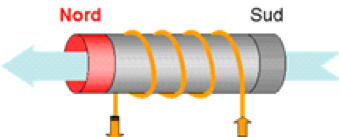
\includegraphics[width=.2\textwidth]{images/indu_aimant1}}
\institute{Lycée Louis Armand}
\date{25 novembre 2018}

\begin{document}
\begin{frame}{}

\end{frame}
    \begin{frame}
        \maketitle
    \end{frame}

    \begin{frame}
        \tableofcontents
    \end{frame}

    \section{Généralités}
    \begin{frame}{La fonction Transmettre}
      \centering
      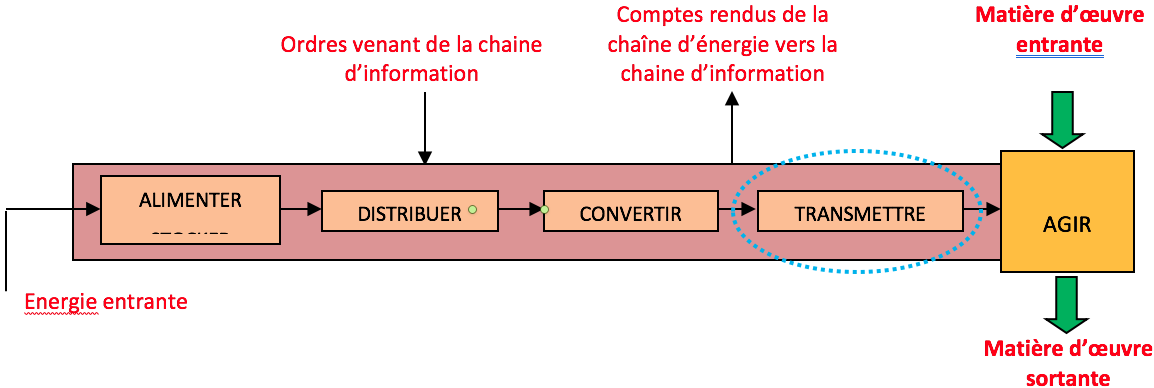
\includegraphics[width=\textwidth]{images/S03_C04}
    \end{frame}

    % \begin{frame}{}
    %   \centering
    %   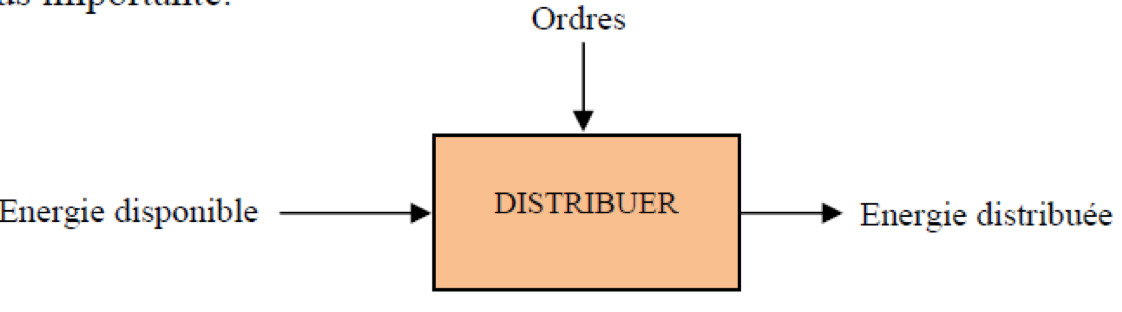
\includegraphics[width=.6\textwidth]{images/distribuer}
    % \end{frame}

    \begin{frame}{Définition}
      \begin{alertblock}{Le bloc transmettre}
        La fonction « Transmettre » permet
        \begin{itemize}
          \item D'adapter l’énergie du point de vue des efforts ou de la vitesse grâce aux réducteurs à engrenage, aux systèmes poulies-courroie ou pignons-chaîne
          \item De transformer l’énergie pour passer d’un type de mouvement à un autre type de mouvement. Par exemple, pour passer d’un mouvement de rotation à un mouvement de translation.
        \end{itemize}

      \end{alertblock}
    \end{frame}

    \begin{frame}{Quelques exemples}
      \centering
      \begin{figure}[h]
        \centering
          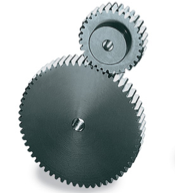
\includegraphics[width=0.24\textwidth]{images/engr_droit}
          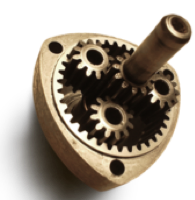
\includegraphics[width=0.24\textwidth]{images/engr_epi}
          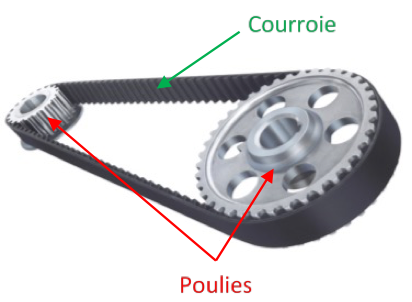
\includegraphics[width=0.24\textwidth]{images/poulie-courroie}
          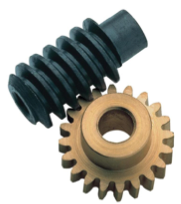
\includegraphics[width=0.24\textwidth]{images/roue_vis}\\

          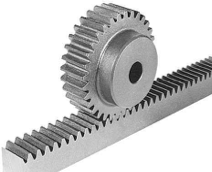
\includegraphics[width=0.24\textwidth]{images/cremaillere}
          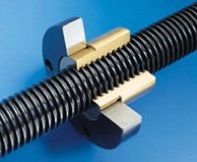
\includegraphics[width=0.24\textwidth]{images/vis_ecrou}
          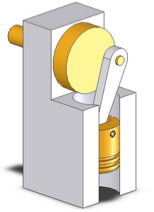
\includegraphics[width=0.24\textwidth]{images/bielle_manivelle}
        \caption{Quelques exemples d'actionneurs}
        \label{fig:exemples}
      \end{figure}
    \end{frame}

\section{Transmission de puissance par engrenages}
\begin{frame}{Définition}
  \centering
  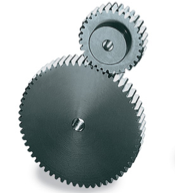
\includegraphics[width=0.3\textwidth]{images/engr_droit}
  \begin{block}{Un engrenage}
    Un engrenage est un système mécanique composé de deux roues dentées qui se transmettent la puissance par obstacle.
    Si un système de transmission par roues dentées est composé de plus de 2 roues alors c’est ce système est un train d’engrenages.
  \end{block}

  \begin{alertblock}{A retenir}
    La roue la plus petite d'un engrenage est appelée un \visible<2>{\alert{pignon}}
  \end{alertblock}
\end{frame}

\begin{frame}[t]{}
  \begin{block}{}
    Le rapport de vitesses angulaires obtenu entre l’entrée et la sortie, également connu sous les dénominations de « \visible<2>{\alert{rapport d'engrenage}} » ou « \visible<2>{\alert{rapport de transmission}} », ne dépend que des nombres de dents des roues en contact. Il est également égal au rapport des rayons, et, a fortiori, des diamètres des roues.
  \end{block}
\end{frame}
%--- Next Frame ---%
%
\begin{frame}
  \begin{itemize}
    \item Une roue droite comporte \trou{un nombre entier de dents}, noté $Z$, placées à intervalles successifs égaux.
    \item La taille de ces intervalles définit le pas $p$ de l'engrenage.
  \end{itemize}

  \begin{alertblock}
    Le rapport $r$, aussi appelé \textit{raison de l'engrenage} est égal à $$r = \frac{Z_{\text{menante}}}{Z_{\text{menante}}} = \frac{\omega_s}{\omega_e}$$

    Avec $Z$ le nombre de dents des roues menante et menée et $\omega_s$ et $\omega_e$ les vitesse d'entrée et de sortie, respectivement.
  \end{alertblock}
\end{frame}

\begin{frame}[t]{Rapport de réduction}
  \begin{block}{Résultat}
    \begin{itemize}
      \item Si $r<1$ \trou{$r$ est un rapport de réduction car la vitesse de sortie est plus faible que la vitesse d'entrée}
      \item Si $r>1$  \trou{$r$ est un rapport de transmission. La vitesse de sortie est plus forte que la vitesse d'entrée. }
      \item Si $r=1$  \trou{La vitesse en entrée est égale à la vitesse en sortie}
    \end{itemize}
  \end{block}
\end{frame}

\begin{frame}[t]{Sens de rotation}
  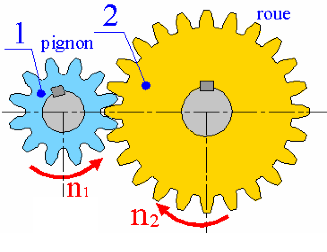
\includegraphics[width=.7\textwidth]{images/engrenage_2_droit}
\end{frame}
%--- Next Frame ---%
\begin{frame}[t]{Puissance et rendement}
  Résultat :
\end{frame}

\section{Engrenage a contact intérieur}
\begin{frame}[t]{Contact interieur}
  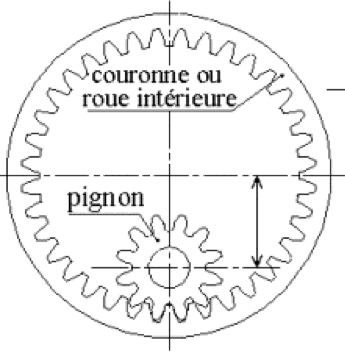
\includegraphics[width=.7\textwidth]{images/engre_interieur}
  Sens de rotation ?
\end{frame}

\begin{frame}[t]{A retenir}
  Le fait que le contact se fasse par l’intérieur n’inverse pas le sens de rotation entre les deux roues.
\end{frame}

\section{Train d'engrenage}
\begin{frame}[t]{Définition}
  \begin{alertblock}{}
    Lorsqu’un système mécanique de transmission est composé de plus de deux roues dentées il est appelé train d’engrenage
  \end{alertblock}
\end{frame}

\begin{frame}[t]{A retenir}

\end{frame}

\begin{frame}[t]{A retenir}
  \begin{description}
    \item [Si n est pair] \trou{Le sens de rotation en sortie est le même que celui en entrée}
    \item [Si n est impair] \trou{Le sens de rotation en sortie est inversé par rapport à celui de l'entrée}
  \end{description}
\end{frame}
%--- Next Frame ---%
%--- Next Frame ---%
%--- Next Frame ---%
%--- Next Frame ---%

%--- Next Frame ---%

%--- Next Frame ---%

%--- Next Frame ---%


    \begin{frame}[focus]
        Questions ?
    \end{frame}

    \appendix
\end{document}
